\documentclass[12pt,letterpaper]{article}
% The usepackage tell LaTeX which packages are needed. As you get better you can add more
% packages for extra functionality
% Percent signs are comments, they will not be read by the renderer.
\usepackage{fullpage}
\usepackage[top=2cm, bottom=2.5cm, left=2.5cm, right=2.5cm]{geometry}
\usepackage{amsmath,amsthm,amsfonts,amssymb,amscd}
\usepackage{lastpage}
\usepackage{enumerate}
\usepackage{fancyhdr}
\usepackage{mathrsfs}
\usepackage{xcolor}
\usepackage{graphicx}
\usepackage{multicol}
\usepackage{wrapfig}
\usepackage{hyperref}
\usepackage{systeme}
\usepackage{subfig}
\usepackage[shortlabels]{enumitem}
\usepackage{listings} %for listings of the source code

% Some definitions for using the listing package.
% When we reference 'codegreen', it will be the RGB color defined below.
\definecolor{codegreen}{rgb}{0,0.6,0}
\definecolor{codegray}{rgb}{0.5,0.5,0.5}
\definecolor{codepurple}{rgb}{0.58,0,0.82}
\definecolor{backcolour}{rgb}{0.95,0.95,0.92}
\DeclareUnicodeCharacter{2212}{-}

% Also for the listings, this will make the code listing look like default MATLAB
\lstdefinestyle{mystyle}{
	backgroundcolor=\color{backcolour},   
	commentstyle=\color{codegreen},
	keywordstyle=\color{magenta},
	numberstyle=\tiny\color{codegray},
	stringstyle=\color{codepurple},
	basicstyle=\footnotesize,
	breakatwhitespace=false,         
	breaklines=true,                 
	captionpos=b,                    
	keepspaces=true,                 
	numbers=left,                    
	numbersep=5pt,                  
	showspaces=false,                
	showstringspaces=false,
	showtabs=false,                  
	tabsize=2
}
\lstset{style=mystyle}

\hypersetup{%
  colorlinks=true,
  linkcolor=blue,
  linkbordercolor={0 0 1}
}
 
\setlength{\parindent}{0.0in}
\setlength{\parskip}{0.05in}

\newcommand\course{COMP 521}
\newcommand\hwnumber{7}             
\newcommand\MyName{Zack Humphries}  

\pagestyle{fancyplain}
\headheight 15pt
\lhead{\MyName}
%\lhead{\NetIDa\\\NetIDb}                 % <-- Comment this line out for problem sets (make sure you are person #1)
\chead{\textbf{\Large Homework \hwnumber}}
\rhead{\course\\ December 2, 2022}
\lfoot{}
\cfoot{}
\rfoot{\small\thepage}
\headsep 1.5em

\begin{document}


\section*{Problem 1}
Solve the one-way wave equation (hyperbolic PDE):

\begin{equation*}
u_t + u_x = 0
\end{equation*}

where


\begin{equation}
u(x,0)=u_0(x) =
\begin{cases}
1 -|x|& \text{if $|x| < 1$ }\\
0 & \text{otherwise}
\end{cases}
\end{equation}\\


\textbf{Use Lax-Friedrichs} with space and time domains of $x \in [-2,10]$ and $t \in [0,8]$ respectively. 
Use left boundary condition $u(-2,t)=u_0 (-2-t)$ and right boundary condition $u(10,t)=u_0 (10-t)$.
\\

\section*{Problem 1: Set Up}
\textbf{Lax-Friedrichs} defines the equation $u_{t} + u_{x} = 0$ as\ldots


\begin{equation*}
    \frac{u^{j+1}_{i} - \frac{1}{2}\left(u^{j}_{i+1} + u^{j}_{i-1}\right)}{\Delta t} + \frac{\left(u^{j}_{i+1} + u^{j}_{i-1}\right)}{2 \Delta t} = 0
\end{equation*}

Factoring out \textbf{$u^{j+1}_{j}$}\ldots

\begin{equation*}
    u^{j+1}_{i} = \frac{1}{2} \left(u^{j}_{i+1} + u^{j}_{i-1}\right) - \frac{\Delta t}{2 \Delta x} \left(u^{j}_{i+1} + u^{j}_{i-1}\right)
\end{equation*}

Defining $r=\frac{\Delta t}{\Delta x}$ and further simplifying, creates the needed finite difference scheme\ldots

\begin{equation*}
    u^{j+1}_{i} = \frac{1-r}{2} \left(u^{j}_{i+1}\right) + \frac{1+r}{2} \left(u^{j}_{i-1}\right)
\end{equation*}

Creating a system of matricies, excluding $u^{j}_{0} = u(-2,t)$ and $u^{j}_{N} = u(10,t)$ from the first and final rows, respectively, leaves\ldots


\begin{equation*}
    \overrightarrow{u}^{j+1}_{i} - \begin{bmatrix} \frac{1+r}{2}u^{j}_{0} \\ 0 \\ \vdots \\ 0 \\ \frac{1-r}{2}u^{j}_{N} \end{bmatrix} = \begin{bmatrix} 0 & \frac{1-r}{2} & 0 & \\ \frac{1+r}{2} & 0 & \frac{1-r}{2} & & \\ 0 & \frac{1+r}{2} & 0 & \ddots & \\ & & \ddots & \ddots & \frac{1-r}{2} \\  & & & \frac{1+r}{2} & 0 \end{bmatrix} \begin{bmatrix} u^{j}_{1} \\ u^{j}_{2} \\ \vdots \\ u^{j}_{N-2} \\ u^{j}_{N-1} \end{bmatrix}
\end{equation*}

For the boundary conditions\: $u(-2,t)=u_0 (-2-t)$ and $u(10,t)=u_0 (10-t)$, given that $t \in [0,8]$, $u_0(-2-t) = 0$ because $|-2-t| > 1$ and $u_0(-2-t) = 0$ because $|10-t| > 1$ for any $t \in [0,8]$, which provides\ldots

\begin{equation*}
    \overrightarrow{u}^{j+1}_{i} = \begin{bmatrix} 0 & \frac{1-r}{2} & 0 & \\ \frac{1+r}{2} & 0 & \frac{1-r}{2} & & \\ 0 & \frac{1+r}{2} & 0 & \ddots & \\ & & \ddots & \ddots & \frac{1-r}{2} \\  & & & \frac{1+r}{2} & 0 \end{bmatrix} \begin{bmatrix} u^{j}_{1} \\ u^{j}_{2} \\ \vdots \\ u^{j}_{N-2} \\ u^{j}_{N-1} \end{bmatrix}
\end{equation*}

\section*{Problem 1: Implementation}

For this problem, I chose my $\Delta x$ as\ldots
\begin{equation*}
    \Delta x = \left[ \left(\frac{1}{2}\right)^{7}, \left(\frac{1}{2}\right)^{8}, \left(\frac{1}{2}\right)^{9}, \left(\frac{1}{2}\right)^{10} \right] 
\end{equation*}
in order to have a more refined error calculation.
\\

I also chose my $\Delta t$, following the Lax-Friedrich CFL, as\ldots
\begin{equation*}
    \Delta t = \frac{\left(\frac{1}{2}\right)^{10}}{2}  \text{\hspace{0.25cm}such that\hspace{0.25cm}} |r| = \left\lvert \frac{\Delta t}{\Delta x}\right\rvert   \leq  1
\end{equation*}
\\

For plotting the numerical vs analytical solution, I chose to plot the Comparison when $t = \left[0,2,4,6,8\right]$
\\

The resulting plots starting on the next page show that numerical result, in blue, follows the analytical result, in red, very well in the beginning. However as the time increases, the numerical and analytical answer begin to separate, especially for the higher $\Delta x$ values.


\newpage


\begin{figure}[!h]
    \centering
    \subfloat{
    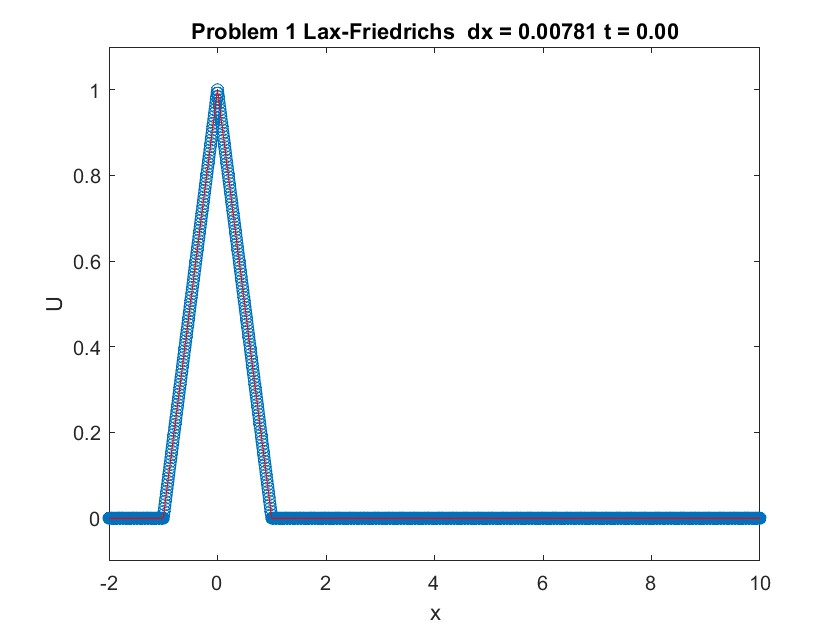
\includegraphics[width=.5\textwidth]{Problem1_1a.jpg}
    }
    \subfloat{
    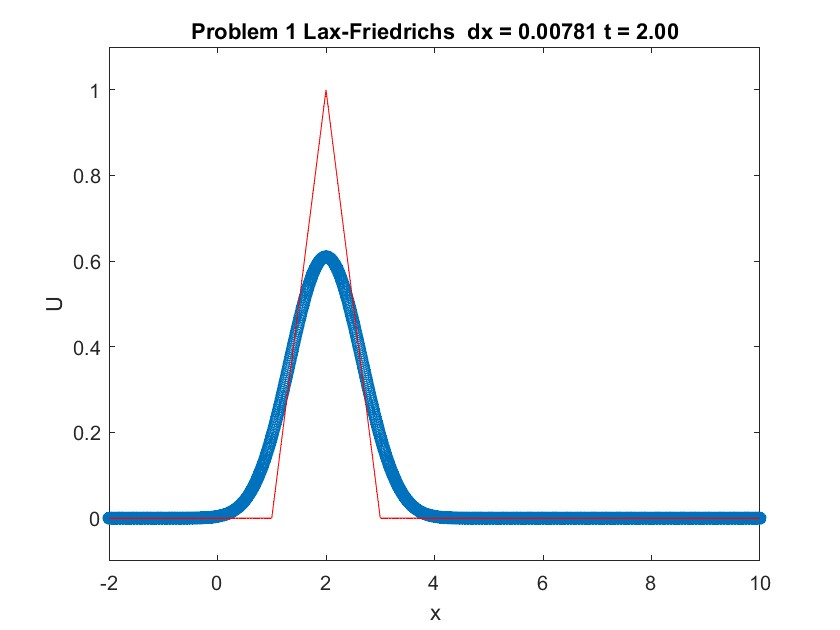
\includegraphics[width=.5\textwidth]{Problem1_1b.jpg}
    }

    \subfloat{
    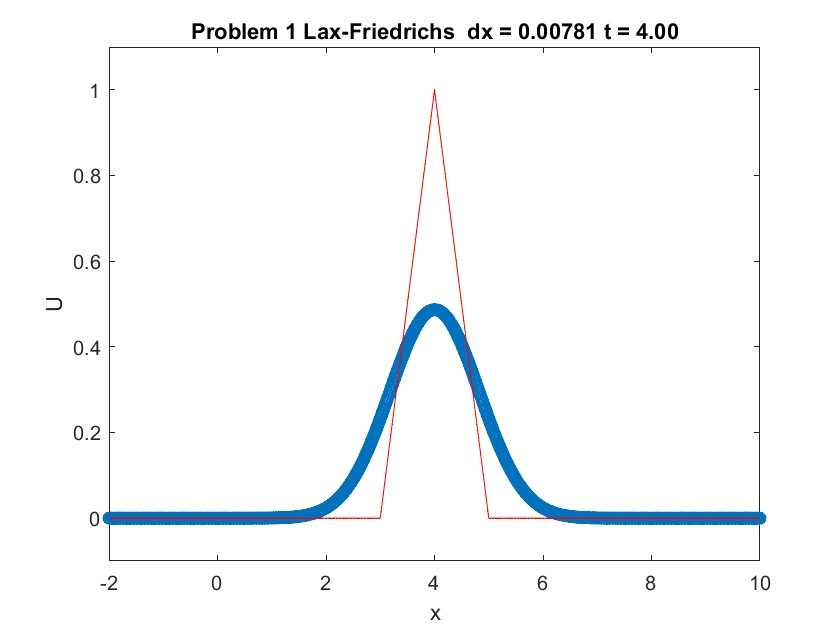
\includegraphics[width=.5\textwidth]{Problem1_1c.jpg}
    }

    \subfloat{
    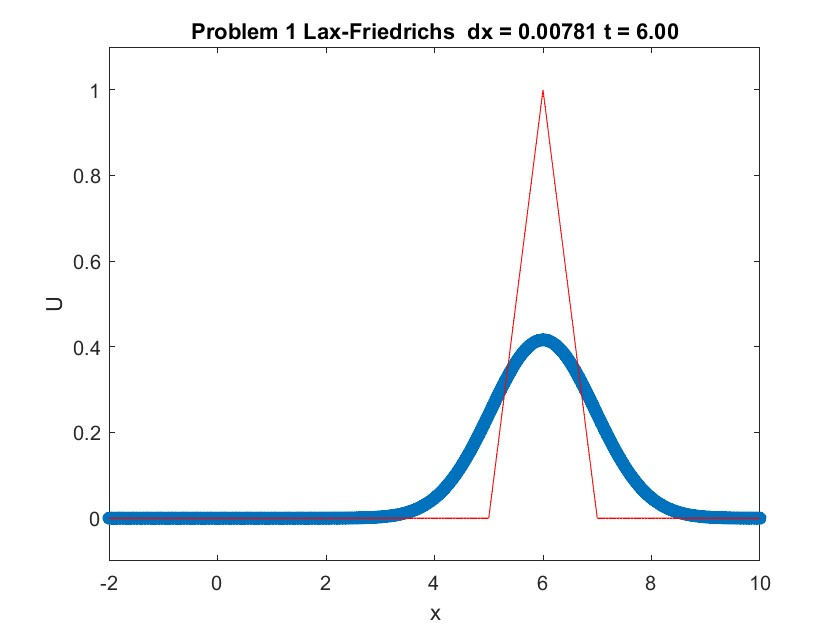
\includegraphics[width=.5\textwidth]{Problem1_1d.jpg}
    }
    \subfloat{
    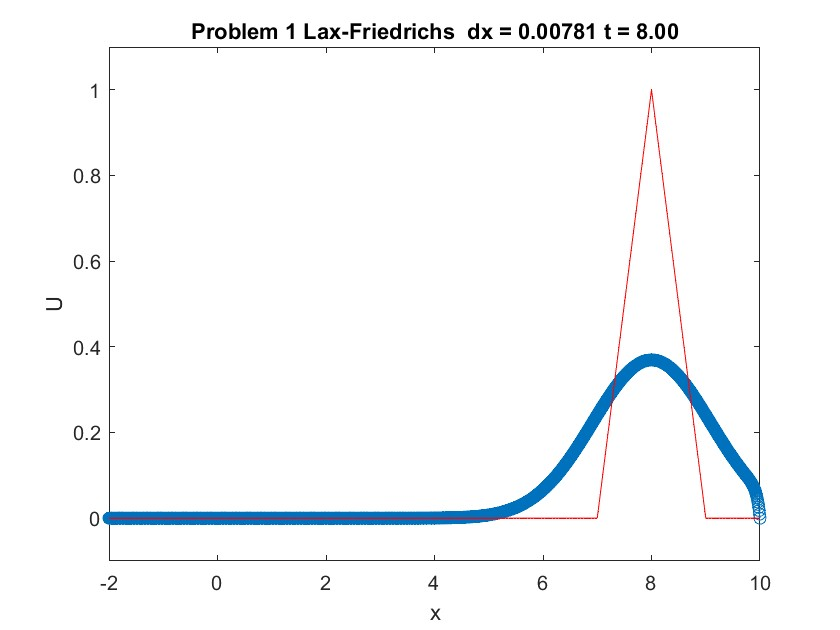
\includegraphics[width=.5\textwidth]{Problem1_1e.jpg}
    }
    
    \caption{$\Delta x =\left(\frac{1}{2}\right)^{7}$}
\end{figure}

\newpage

\begin{figure}[!h]
    \centering
    \subfloat{
    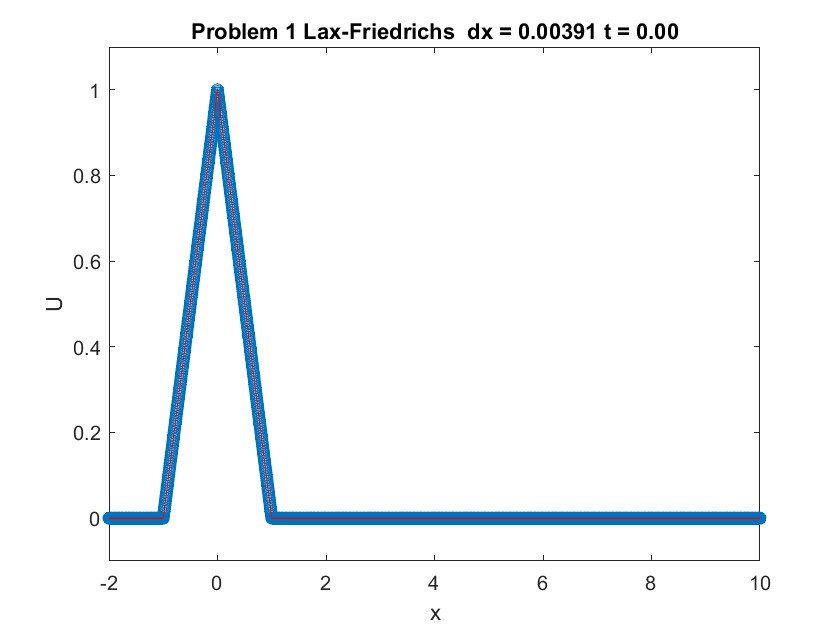
\includegraphics[width=.5\textwidth]{Problem1_2a.jpg}
    }
    \subfloat{
    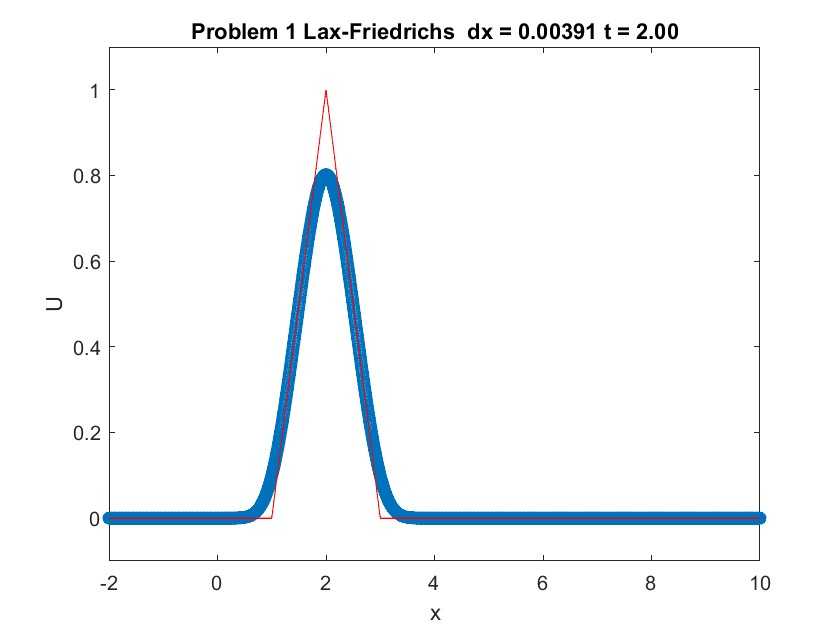
\includegraphics[width=.5\textwidth]{Problem1_2b.jpg}
    }

    \subfloat{
    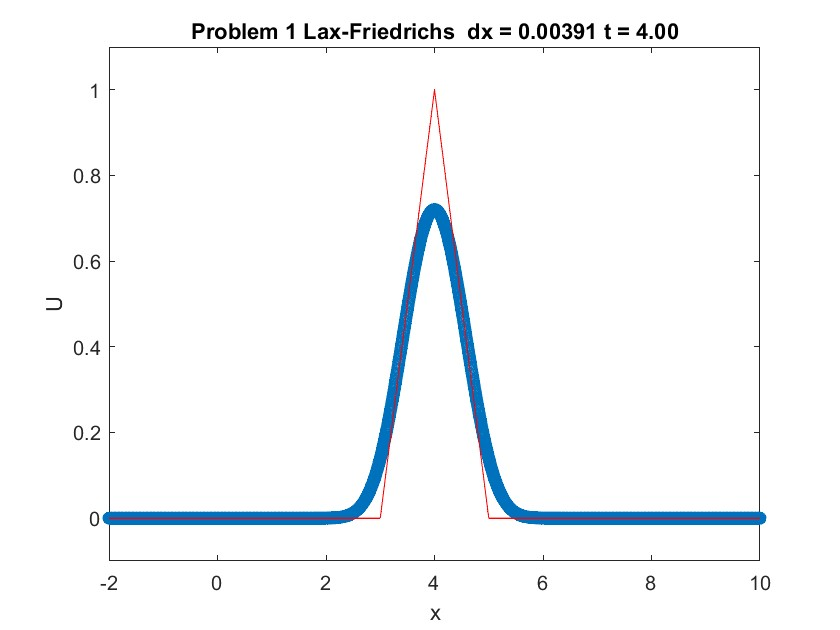
\includegraphics[width=.5\textwidth]{Problem1_2c.jpg}
    }

    \subfloat{
    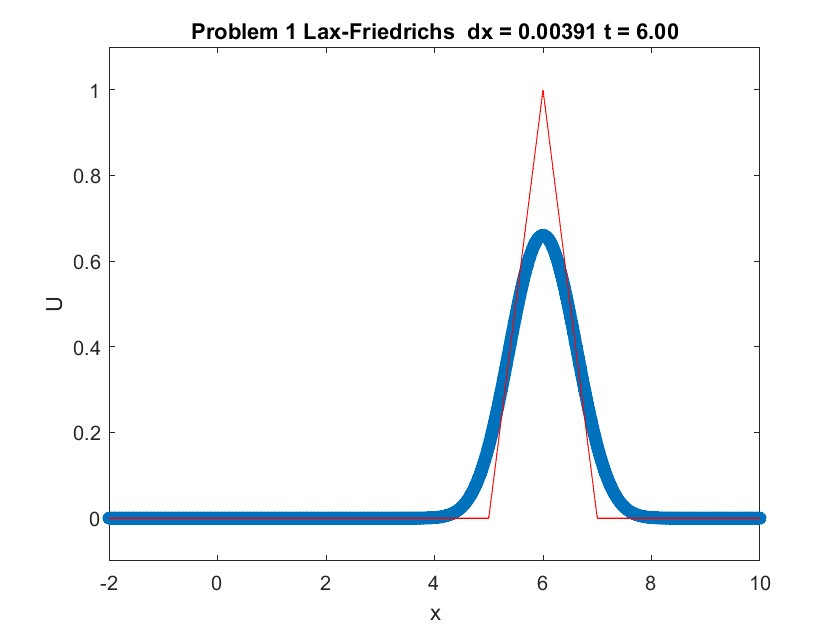
\includegraphics[width=.5\textwidth]{Problem1_2d.jpg}
    }
    \subfloat{
    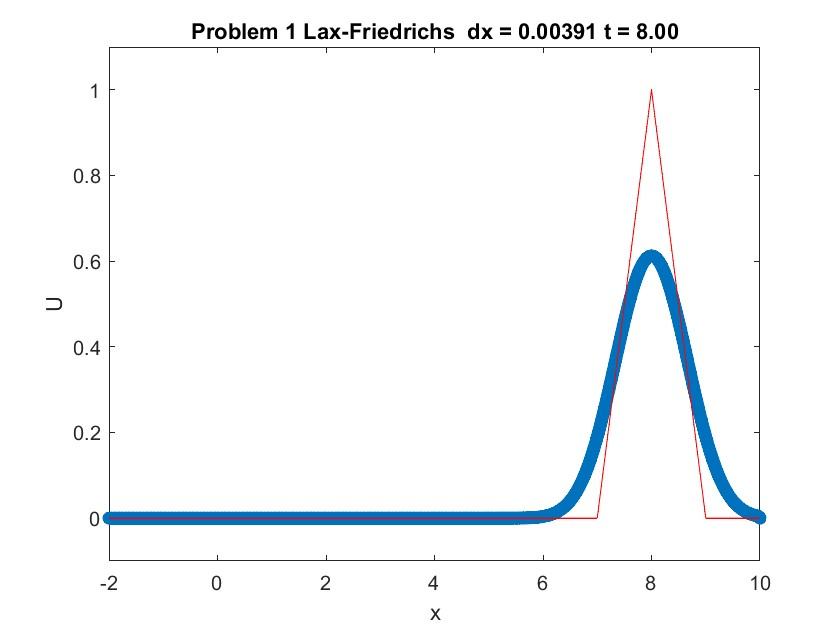
\includegraphics[width=.5\textwidth]{Problem1_2e.jpg}
    }
    
    \caption{$\Delta x =\left(\frac{1}{2}\right)^{8}$}
\end{figure}

\newpage

\begin{figure}[!h]
    \centering
    \subfloat{
    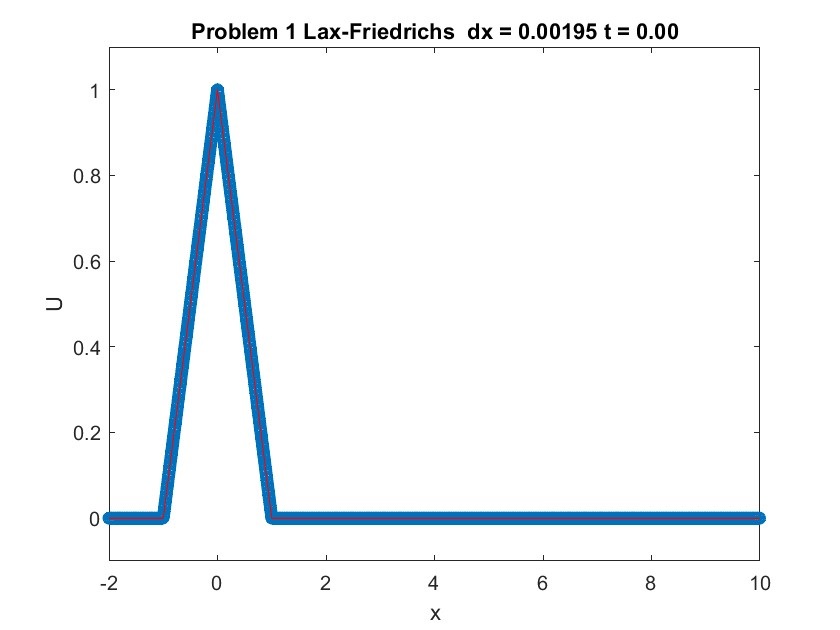
\includegraphics[width=.5\textwidth]{Problem1_3a.jpg}
    }
    \subfloat{
    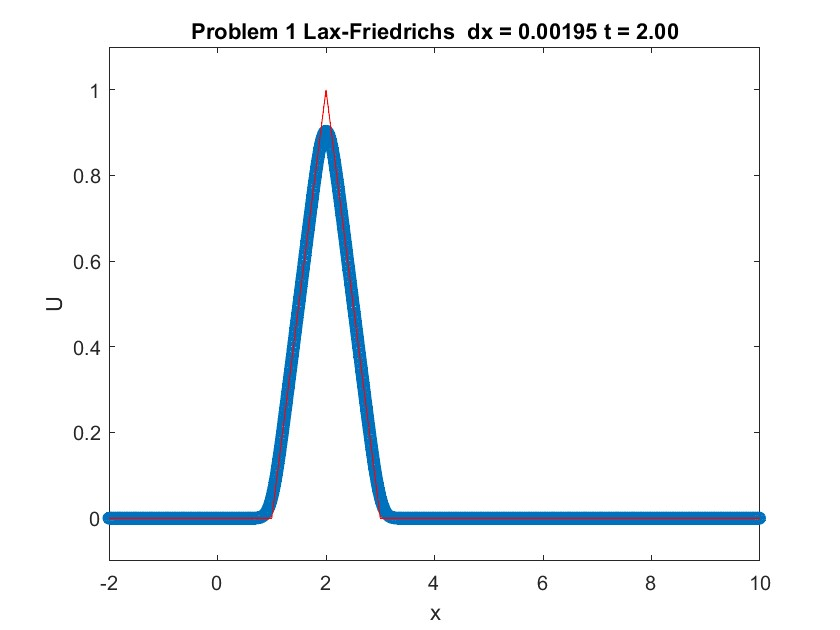
\includegraphics[width=.5\textwidth]{Problem1_3b.jpg}
    }

    \subfloat{
    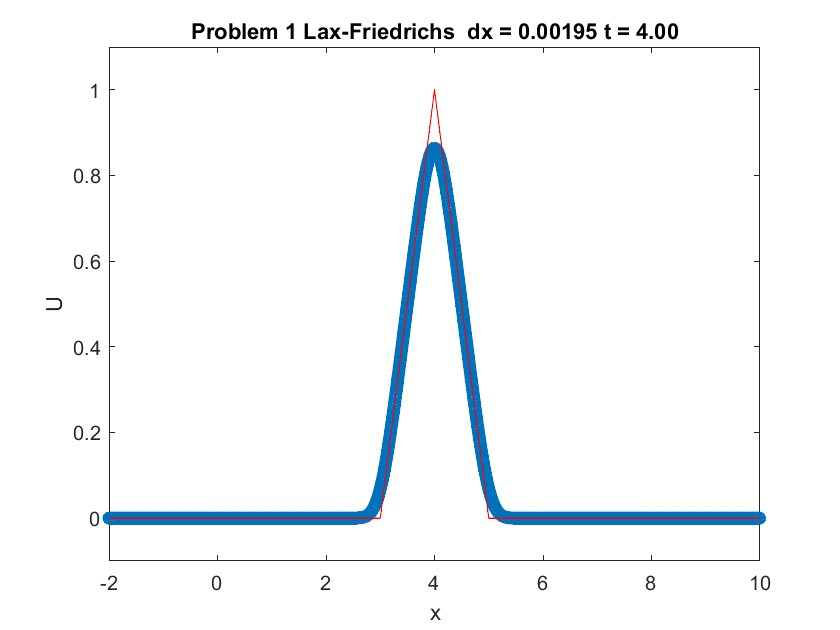
\includegraphics[width=.5\textwidth]{Problem1_3c.jpg}
    }

    \subfloat{
    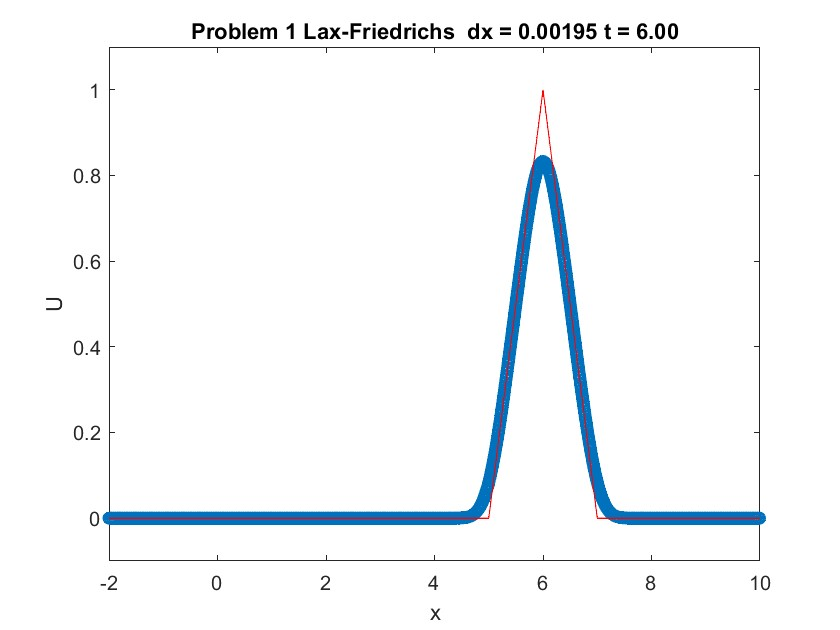
\includegraphics[width=.5\textwidth]{Problem1_3d.jpg}
    }
    \subfloat{
    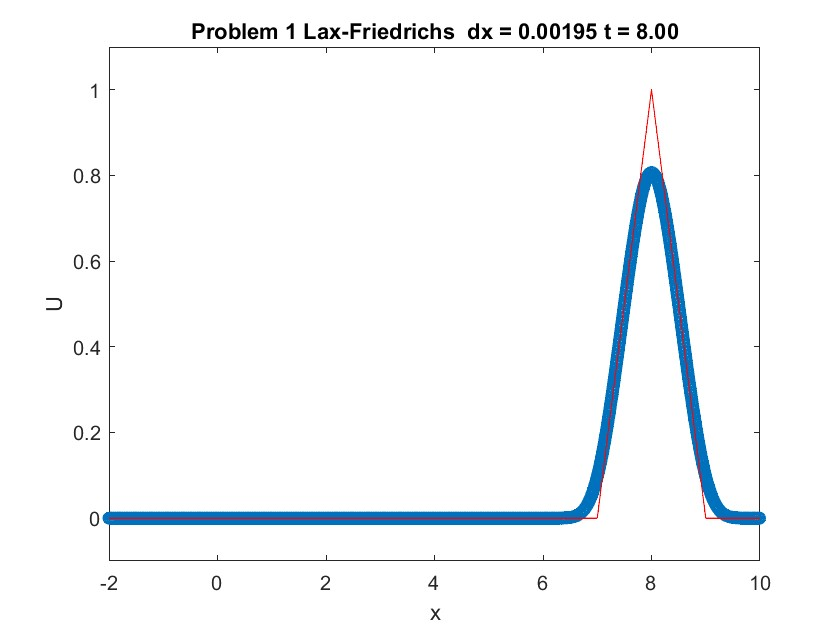
\includegraphics[width=.5\textwidth]{Problem1_3e.jpg}
    }
    
    \caption{$\Delta x =\left(\frac{1}{2}\right)^{9}$}
\end{figure}

\newpage

\begin{figure}[!h]
    \centering
    \subfloat{
    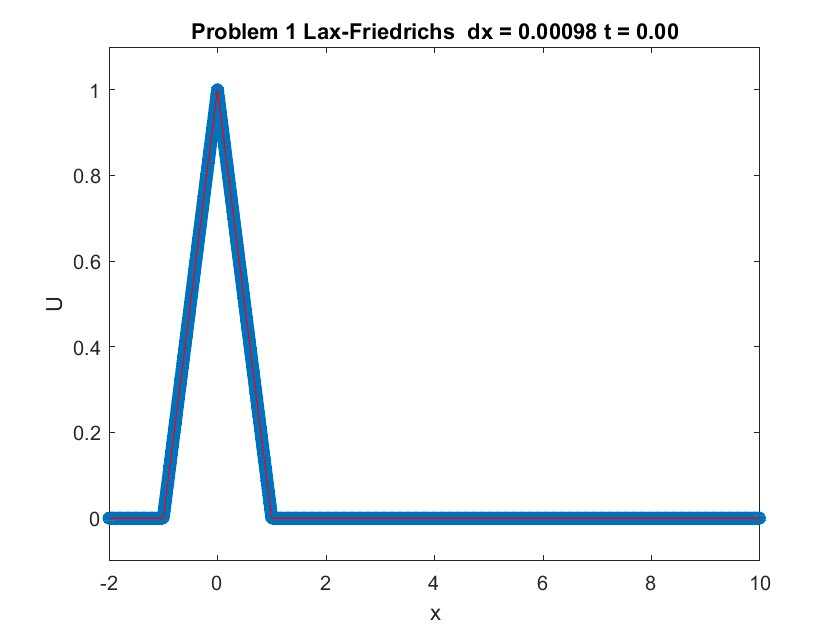
\includegraphics[width=.5\textwidth]{Problem1_4a.jpg}
    }
    \subfloat{
    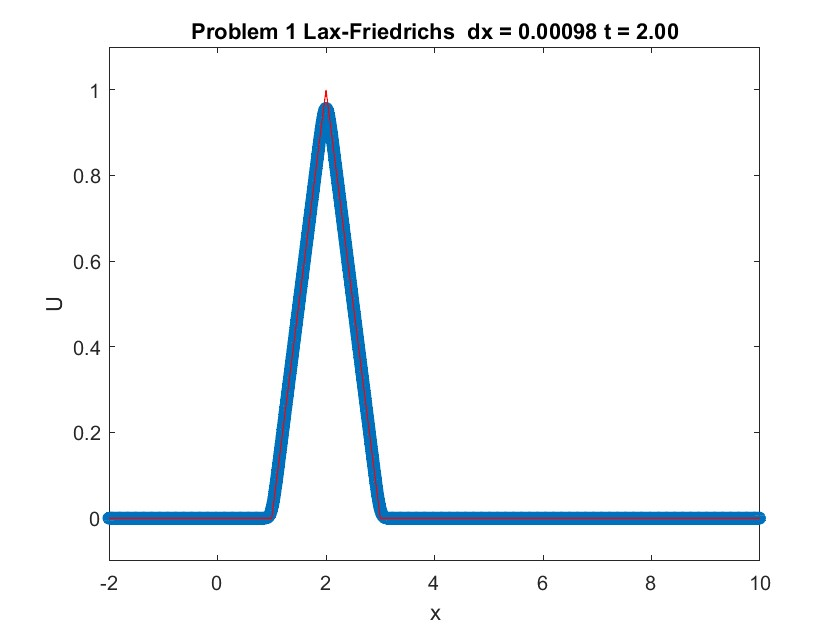
\includegraphics[width=.5\textwidth]{Problem1_4b.jpg}
    }

    \subfloat{
    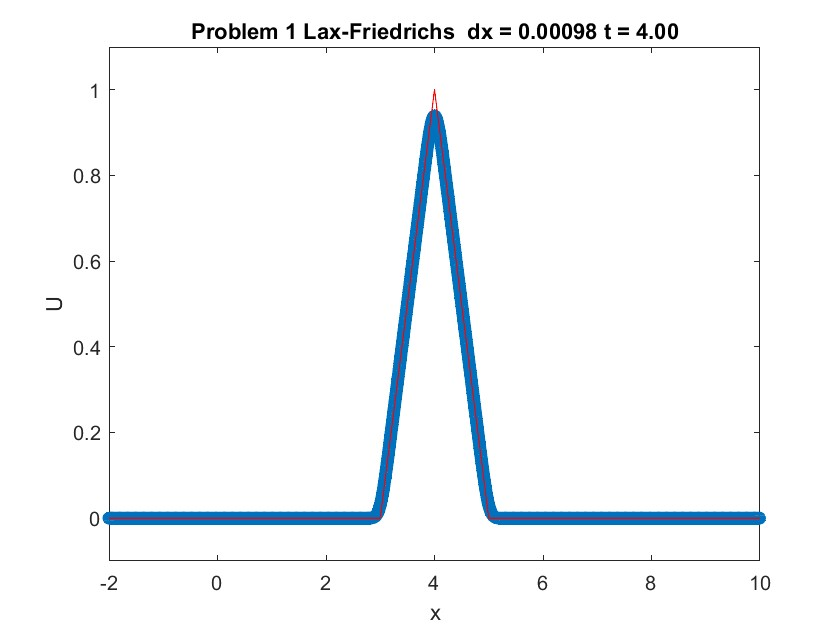
\includegraphics[width=.5\textwidth]{Problem1_4c.jpg}
    }

    \subfloat{
    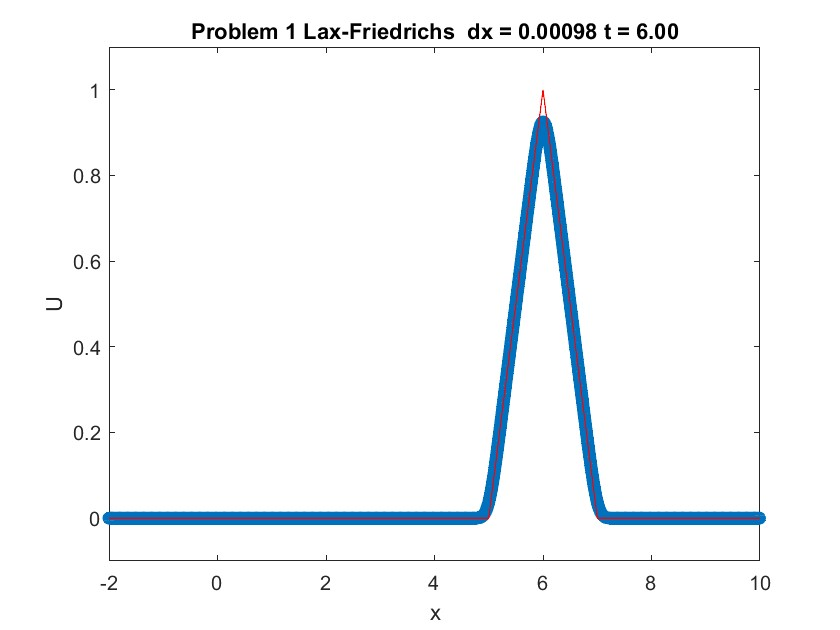
\includegraphics[width=.5\textwidth]{Problem1_4d.jpg}
    }
    \subfloat{
    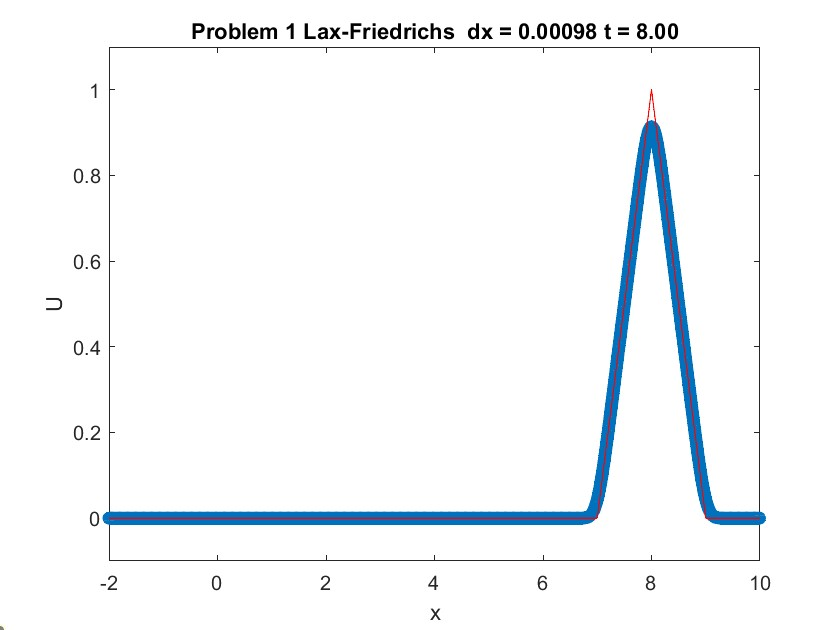
\includegraphics[width=.5\textwidth]{Problem1_4e.jpg}
    }
    
    \caption{$\Delta x =\left(\frac{1}{2}\right)^{10}$}
\end{figure}

\newpage


\section*{Problem 1: Error Analysis}

Per instructions, the error is calculated at the final time step $t=8$. I am using the same list of $\Delta x$ values as well.
\\

One thing to note is that I decided that the best place calculate the error would be at when $x = 8$. This is because the peak of the wave is at $x = 8$ at $t = 8$, thus being a good place to calculate the accuracy of the scheme.


\begin{figure}[!h]
    \centering
    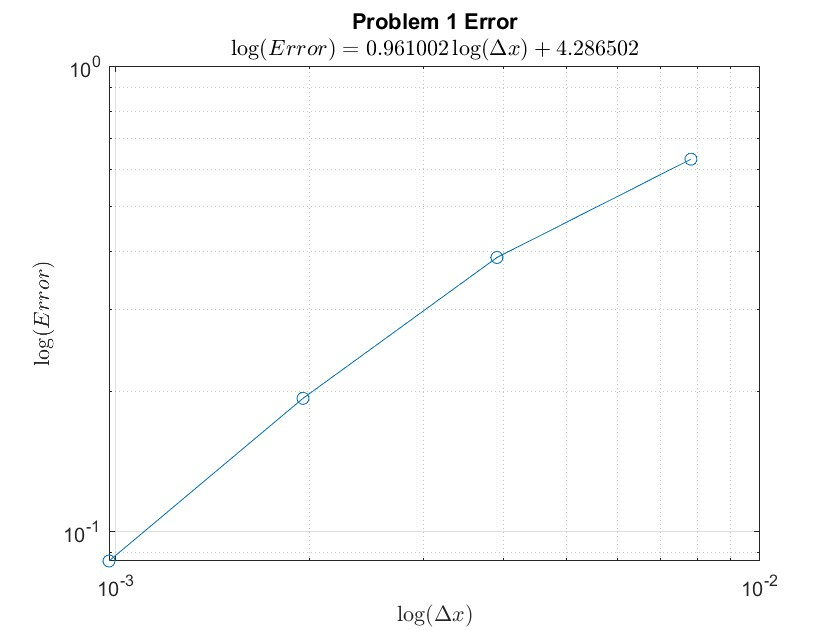
\includegraphics[width = 0.9\textwidth]{Problem1_Error.jpg}

    \caption{Problem 1 LogLog Plot of Error}

\end{figure}

The plot shows that the spacial error of this scheme is one with the coefficient of the loglog plot being one.


\newpage

\lstset{title={Problem 1 Matlab Code}}
\begin{lstlisting}[language = Matlab]
%% HW 7
% Zachary Humphries
% COMP 521
% Fall 2022

clc
clear
close all

%% Problem 1

a = -2;         % Left Boundary (x)
b = 10;         % Right Boundary (x)

T = 8;          % Final Time
plot_list = [T/4, T/2, 3*T/4, T];

dx_list = [0.5^7, 0.5^8, 0.5^9, 0.5^10];
dt = dx_list(end)/2;   % To meet condition of |r| <= 1
error_list = zeros(length(dx_list), 1);

for i=1:length(dx_list)
    dx = dx_list(i);
    xgrid_short = [a+dx:dx:b-dx];
    xgrid_long = [a:dx:b];
    
    ICV = xgrid_short';
    ICV = problem1_u0(ICV);

    left_boundary = 0;
    right_boundary = 0;

    r=dt/dx;

    U = ICV;

    actual = problem1_u0(0-xgrid_long);

    figure(1+(5*(i-1)))
    plot([a xgrid_short b], [left_boundary U' right_boundary] , 'o-')
    hold on
    plot([xgrid_long], [actual] , 'r-')
    axis([a b -0.1 1.1])
    str = sprintf('Problem 1 Lax-Friedrichs \t dx = %.5f t = %.2f', dx, 0.0);
    title(str)
    xlabel('x')
    ylabel('U')
    hold off

    A = problem1_matrix(a,b,dx,dt);

    for dt_j = dt: dt : T
        left_boundary = problem1_u0(-2-dt_j);
        right_boundary = problem1_u0(10-dt_j);


        U(1) = U(1);
        U(end) = U(end);

        U = A*U;

        actual = problem1_u0(dt_j-xgrid_long);
        for k=1:length(plot_list)
            if (dt_j == plot_list(k))
                figure(1+k+(5*(i-1)))
                plot([a xgrid_short b], [left_boundary U' right_boundary] , 'o-')
                hold on
                plot([xgrid_long], [actual] , 'r-')
                axis([a b -0.1 1.1])
                str = sprintf('Problem 1 Lax-Friedrichs \t dx = %.5f t = %.2f', dx, dt_j);
                title(str)
                xlabel('x')
                ylabel('U')
                hold off
                pause(0.1)
            end
        end
    end
    index_actual = find(xgrid_long(1, :) == 8);
    index_U = find(xgrid_short(1, :) == 8);
    error_list(i,1) = abs(U(index_U,1) - actual(1,index_actual));
end

figure
forward_poly = polyfit(log(dx_list), log(error_list), 1);
loglog(dx_list, error_list, "o-"); grid on;
title("Problem 1 Error")
subtitle_name_forward = strcat("$\log(Error) = ", sprintf("%2.6f", forward_poly(1)), "\log(\Delta x) + ", sprintf("%2.6f", forward_poly(2)), "$");
subtitle(subtitle_name_forward,'interpreter','latex')
xlabel("$\log(\Delta x)$",'interpreter','latex')
ylabel("$\log(Error)$",'interpreter','latex')



function A = problem1_matrix(a,b,dx,dt)
    r = dt/dx;
    m = (b-a)/dx;
    one = ones(m-1,1);
    diag1 = (1+r)/2 * one;
    diag2 = (1-r)/2 * one;

    A = spdiags([diag1 zeros(m-1,1) diag2],-1:1,m-1,m-1);
    A = sparse(A);
end

function u0x = problem1_u0(x)
    u0x = zeros(size(x));
    for i=1:length(x)
        if abs(x(i)) <1
            u0x(i) = 1-abs(x(i));
        else
            u0x(i) = 0;
        end
    end
end
\end{lstlisting}


\newpage

\section*{Problem 2}

Find the numerical solution for the following heat equation:

\begin{equation*}
u_t + u_{xx} = 0 \quad  \text{for} \quad 0<x<1 \quad \text{and} \quad 0 \le t \le 0.1
\end{equation*}

with the initial condition  $u(x,0)= f(x)= sin(\pi x)+ sin(3\pi x) \quad  \forall x \in [0,1]$ and boundary conditions:
\begin{center}
    $ u(0,t) = c_1 = 0 \quad$ for $\quad x=0 \quad$ and $\quad 0\le t \le 0.1 $ \\
    $ u(1,t) = c_2 = 0 \quad$ for $\quad x=1 \quad$ and $\quad 0\le t \le 0.1 $ 
\end{center}


The exact solution is\: 
\begin{equation*}
    u(x,t) = sin(\pi x)e^{-\pi^2t} + sin(3\pi x)e^{-9\pi^2t}
\end{equation*}



\section*{Problem 2: Set Up}

The explicit scheme used in class for the heat equation $u_t = c^2 u_{tt}$ as\ldots

\begin{equation*}
    \frac{u^{j+1}_{i}-u^{j}_{i}}{\Delta t} = c^2 \frac{u^{j}_{i-1}-2u^{j}_{i}+u^{j}_{i+1}}{\Delta x^2}
\end{equation*}

Since $c=1$, solving for $u^{j+1}_{i}$ the equation is rewritten as\ldots

\begin{equation*}
    u^{j+1}_{i} = u^{j}_{i} + r\left(u^{j}_{i-1}-2u^{j}_{i}+u^{j}_{i+1}\right) \\
    \quad \text{with} \quad r = \frac{\Delta t}{\Delta x^2}
\end{equation*}

Creating a system of matricies, excluding $u^{j}_{0} = u(0,t) = 0$ and $u^{j}_{N} = u(1,t) = 0$ from the first and final rows, respectively, leaves\ldots


\begin{equation*}
    \overrightarrow{u}^{j+1}_{i} - \begin{bmatrix} ru^{j}_{0} \\ 0 \\ \vdots \\ 0 \\ ru^{j}_{N} \end{bmatrix} = \begin{bmatrix} 1-2r & r & 0 & \\ r & 1-2r & r & & \\ 0 & r & 1-2r & \ddots & \\ & & \ddots & \ddots & r \\  & & & r & 1-2r \end{bmatrix} \begin{bmatrix} u^{j}_{1} \\ u^{j}_{2} \\ \vdots \\ u^{j}_{N-2} \\ u^{j}_{N-1} \end{bmatrix}
\end{equation*}


Given that the boundary conditions $u^{j}_{0} = u(0,t) = 0$ and $u^{j}_{N} = u(1,t) = 0$ for any $t \in [0,0.1]$, $ru^{j}_{0}$ and $ru^{j}_{N}$ can be eliminated providing\ldots

\begin{equation*}
    \overrightarrow{u} ^{j+1}_{i} = \begin{bmatrix} 1-2r & r & 0 & \\ r & 1-2r & r & & \\ 0 & r & 1-2r & \ddots & \\ & & \ddots & \ddots & r \\  & & & r & 1-2r \end{bmatrix} \begin{bmatrix} u^{j}_{1} \\ u^{j}_{2} \\ \vdots \\ u^{j}_{N-2} \\ u^{j}_{N-1} \end{bmatrix}
\end{equation*}


\section*{Problem 2: Implementation with $\Delta x = 0.2$ and $\Delta t = 0.02$}

3D mesh plots showing the numerical and exact results through time, as well as the error between the two are below\:

\begin{figure}[!h]
    \centering
    \subfloat{
    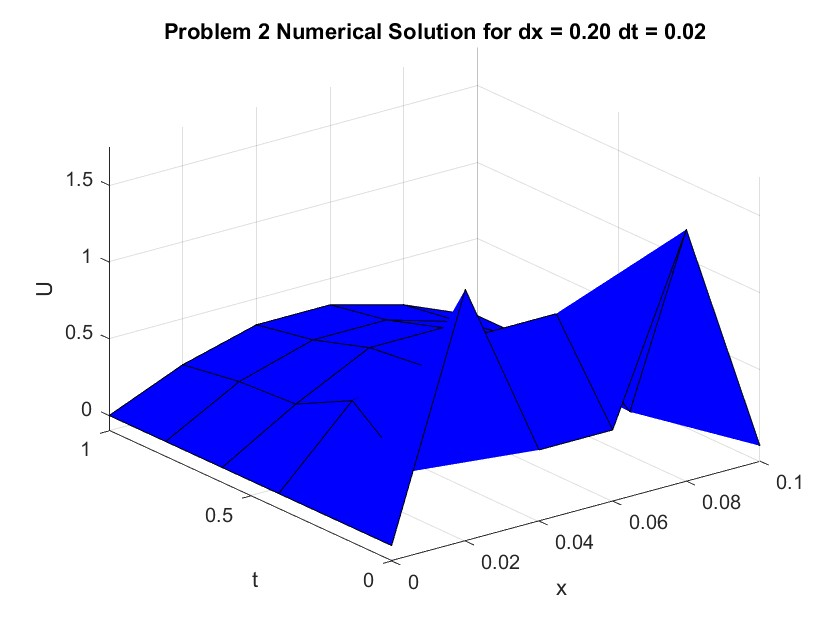
\includegraphics[width=.5\textwidth]{Problem2_a1.jpg}
    }
    \subfloat{
    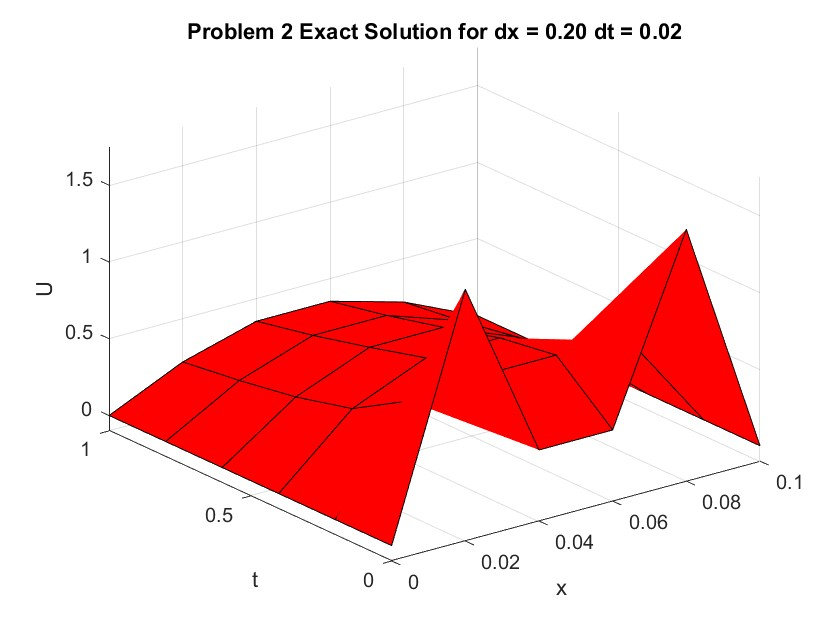
\includegraphics[width=.5\textwidth]{Problem2_a2.jpg}
    }

    \subfloat{
    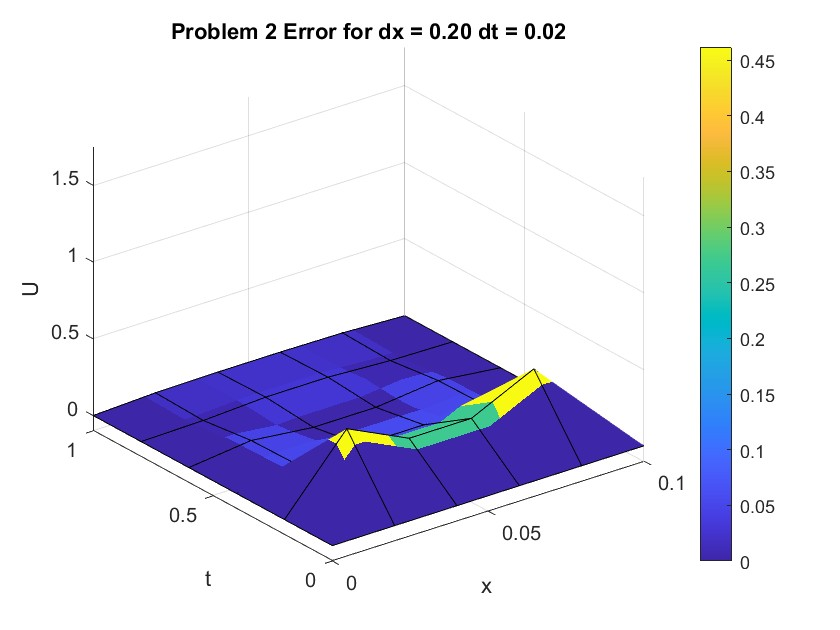
\includegraphics[width=.75\textwidth]{Problem2_a3.jpg}
    }
    
    \caption{Problem 2 with $\Delta x = 0.2$ and $\Delta t = 0.02$}
\end{figure}

With a rather large $\Delta x$ and $\Delta t$, there is a greater error between the numerical and exact results towards the beginning, \\ 
However, as the heat dissipates to $u=0$ through time, the two results begin to allign with a lower error.

\section*{Problem 2: Error Analysis}

For this problem, I chose my $\Delta x$ as\ldots
\begin{equation*}
    \Delta x = \left[ \left(\frac{1}{2}\right)^{3}, \left(\frac{1}{2}\right)^{4}, \left(\frac{1}{2}\right)^{5}, \left(\frac{1}{2}\right)^{6}, \left(\frac{1}{2}\right)^{7} \right] 
\end{equation*}
in order to have a more refined error calculation.
\\

I also chose my $\Delta t$, following the Von Neumann stability criterion, as\ldots
\begin{equation*}
    \Delta t = \frac{\left(\left(\frac{1}{2}\right)^{7}\right)^2}{4} \text{\hspace{0.25cm}such that\hspace{0.25cm}} |r| = \left\lvert \frac{\Delta t}{\Delta x^2}\right\rvert   \leq  \frac{1}{2}
\end{equation*}

One last thing to note is that I chose the midpoint at the final iteration, $t=0.1$ and $x = 0.5$, as my value to do the error analysis.

A log-log plot showing the error of the scheme with differing $\Delta x$ is shown below\ldots

\begin{figure}[!h]
    \centering
    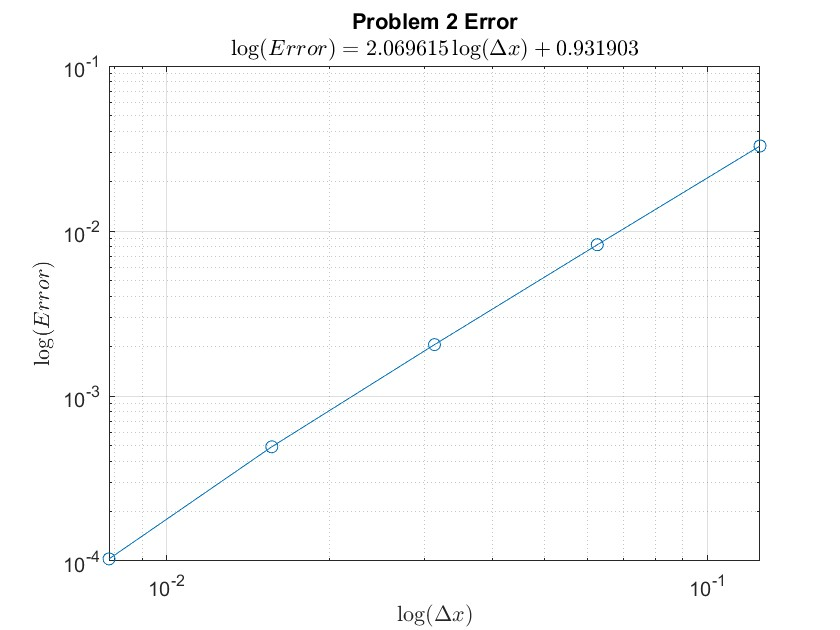
\includegraphics[width = 0.9\textwidth]{Problem2_b.jpg}

    \caption{Problem 2 LogLog Plot of Error}

\end{figure}


The plot shows that the spacial accuracy of this scheme is two with the coefficient of the loglog plot being two.

\newpage

\lstset{title={Problem 2 Matlab Code}}
\begin{lstlisting}[language = Matlab]
%% HW 7
% Zachary Humphries
% COMP 521
% Fall 2022

clc
clear
close all

%% Problem 2

a = 0;         % Left Boundary (x)
b = 1;         % Right Boundary (x)

T = 0.1;          % Final Time

%% a)

dx_list = 0.2;
dt = 0.02;

estimated_U = zeros(length([0:dt:T]), length([a:dx_list:b]));
actual_U = zeros(length([0:dt:T]), length([a:dx_list:b]));


for i=1:length(dx_list)
    dx = dx_list(i);
    xgrid_short = [a+dx:dx:b-dx];
    xgrid_long = [a:dx:b];
    
    ICV = xgrid_short';
    ICV = problem2_u0(ICV,0);

    left_boundary = 0;
    right_boundary = 0;

    r=dt/(dx^2);

    U = ICV;
    estimated_U(1, :) = [left_boundary U' right_boundary];

    actual = problem2_u0(xgrid_long, 0);
    actual_U(1, :) = actual;

    A = problem2_matrix(a,b,dx,dt);

    count = 2;

    for dt_j = dt: dt : T

        U(1) = U(1);
        U(end) = U(end);

        U = A*U;

        actual = problem2_u0(xgrid_long, dt_j);
        actual_U(count, :) = actual;

        estimated_U(count, :) = [left_boundary U' right_boundary];
        
        count = count +1;
    end
end

[X_mesh, T_mesh] = meshgrid([a:dx:b] , [0:dt:T]);


mesh(X_mesh, T_mesh, estimated_U, 'FaceColor','b', 'EdgeColor', "k")
title([sprintf('Problem 2 Numerical Solution for dx = %.2f dt = %.2f', dx_list, dt)])
xlabel('x')
ylabel('t')
zlabel('U')
axis([a b, 0, T, -0.1 1.75])
drawnow

figure
mesh(X_mesh, T_mesh, (actual_U), 'FaceColor','r', 'EdgeColor', "k")
title([sprintf('Problem 2 Exact Solution for dx = %.2f dt = %.2f', dx_list, dt)])
xlabel('x')
ylabel('t')
zlabel('U')
axis([a b, 0, T, -0.1 1.75])
drawnow

figure
mesh(X_mesh, T_mesh, (abs(actual_U-estimated_U)), 'FaceColor','texturemap', 'EdgeColor', "k")
title([sprintf('Problem 2 Error for dx = %.2f dt = %.2f', dx_list, dt)])
xlabel('x')
ylabel('t')
zlabel('U')
axis([a b, 0, T, -0.1 1.75])
colorbar
caxis([0, max(abs(actual_U-estimated_U), [], 'all')])
drawnow

%% b)

% If you want plots similar to (a), uncomment the code below

dx_list = [0.5^3, 0.5^4, 0.5^5, 0.5^6, 0.5^7];
dt = dx_list(end)^2/4;

error_list = zeros(length(dx_list), 1);

for i=1:length(dx_list)
    dx = dx_list(i);
    xgrid_short = [a+dx:dx:b-dx];
    xgrid_long = [a:dx:b];

%     estimated_U = zeros(length([0:dt:T]), length([a:dx:b]));
%     actual_U = zeros(length([0:dt:T]), length([a:dx:b]));
    
    ICV = xgrid_short';
    ICV = problem2_u0(ICV,0);

    left_boundary = 0;
    right_boundary = 0;

    r=dt/(dx^2);

    U = ICV;

    actual = problem2_u0(xgrid_long, 0);

%     actual_U(1, :) = actual;
% 
%     estimated_U(1, :) = [left_boundary U' right_boundary];

    A = problem2_matrix(a,b,dx,dt);

    count = 2;

    for dt_j = dt: dt : T

        U(1) = U(1);
        U(end) = U(end);

        U = A*U;

        actual = problem2_u0(xgrid_long, dt_j);

%         actual_U(count, :) = actual;
%         estimated_U(count, :) = [left_boundary U' right_boundary];

        count = count+1;
    end

    error_list(i,1) = abs(U(((length(U)+1)/2),1)-actual(1,((length(U)+1)/2)));



%     [X_mesh, T_mesh] = meshgrid([a:dx:b] , [0:dt:T]);
% 
%     figure
%     mesh(X_mesh, T_mesh, estimated_U, 'FaceColor','b')
%     title([sprintf('Problem 2 Numerical Solution for dx = %.5f dt = %.5f', dx, dt)])
%     xlabel('x')
%     ylabel('t')
%     zlabel('U')
%     axis([a b, 0, T, -0.1 1.75])
%     drawnow
%     
%     figure
%     mesh(X_mesh, T_mesh, (actual_U), 'FaceColor','r')
%     title([sprintf('Problem 2 Exact Solution for dx = %.5f dt = %.5f', dx, dt)])
%     xlabel('x')
%     ylabel('t')
%     zlabel('U')
%     axis([a b, 0, T, -0.1 1.75])
%     drawnow
%     
%     figure
%     mesh(X_mesh, T_mesh, (abs(actual_U-estimated_U)), 'FaceColor','texturemap', 'EdgeColor', "none")
%     title([sprintf('Problem 2 Error for dx = %.5f dt = %.5f', dx, dt)])
%     xlabel('x')
%     ylabel('t')
%     zlabel('U')
%     axis([a b, 0, T, 0, max(abs(actual_U-estimated_U), [], 'all')])
%     colorbar
%     caxis([0, max(abs(actual_U-estimated_U), [], 'all')])
%     drawnow

end

figure
forward_poly = polyfit(log(dx_list), log(error_list), 1);
loglog(dx_list, error_list, "o-"); grid on;
title("Problem 2 Error")
subtitle_name_forward = strcat("$\log(Error) = ", sprintf("%2.6f", forward_poly(1)), "\log(\Delta x) + ", sprintf("%2.6f", forward_poly(2)), "$");
subtitle(subtitle_name_forward,'interpreter','latex')
xlabel("$\log(\Delta x)$",'interpreter','latex')
ylabel("$\log(Error)$",'interpreter','latex')

function A = problem2_matrix(a,b,dx,dt)
    r = dt/(dx^2);
    m = (b-a)/dx;
    one = ones(m-1,1);
    diag1 = r * one;
    diag2 = (1-2*r) * one;

    A = spdiags([diag1 diag2 diag1],-1:1,m-1,m-1);
    A = sparse(A);
end

function u0x = problem2_u0(x, time)
    u0x = (sin(pi*x)*exp(-pi^2 *time))+(sin(3*pi*x)*exp(-9*pi^2 *time));
end
\end{lstlisting}




\end{document}